
\subsection{Transformer Core Measurements}
In second approach, the witness cylinder was used as the core of a
transformer. Two coils (primary and sense coils) were wound on the
witness cylinder using copper wire. For this technique, three witness cylinder used and each had different number of winding on primary and secondary coil. This enabled more saturation of the material. The primary coil generated an AC magnetic field
using the internal oscillator of a SRS830 lock-in amplifier while the
sense coil measured the sense voltage and picked up the magnetic
field flux produced by the primary coil. This experiment was done at 1
Hz and as small as possible $H$, the order of 0.1~A/m,
% state typical value
to measure the slope of the minor $B-H$ loops near the origin of the
$B-H$ space. In lower frequencies, noise dominated the actual signal.
% why?

The temperature of the core was measured at the same time as the sense voltage by using non-magnetic type T thermocouples. The measured voltage induced on the sense coil, is proportional to $\mu$.  
%The measurements show a range of 0.1\%/K to 2\%/K for $\frac{1}{\mu}\frac{d\mu}{dT}$, again assuming the material to be linear.

In all transformer measurements, the sense voltage from the sense coil
was demodulated by a lock-in amplifier. In
Fig.~\ref{fig:data_and_simulation} the in-phase component $Y$ and
out-of-phase component $X$ of the sense signal as a function of
applied $H$ field at 1 Hz are shown. In the ideal case where the
material is linear, the $X$ component should be zero. But our observation showed a nonzero value for the $X$ component at all frequencies at a typical applied $H$ field. At higher frequencies the value of $X$ dominates the measured signal.
Therefore, the ratio of $X/Y$ depends on both the applied frequency and the position on the
$B-H$ region. We were interested in regions where $\vert Y \vert >
\vert X \vert $ in which the material behaves as being linear and the
$\vert H \vert $ values correspond to $\vert X \vert < \vert X_{max}
\vert$ while still being able to get a good signal to noise ratio.


%A concern in both measurements is that, the material is not linear. 
The observation of nonzero $X$ signal is due to effects such as the nonlinearity of the witness cylinders, such as hysteresis, saturation, eddy currents and skin depth. Therefore, it is not possible to embody the results as a single parameter.
To check the sensitivity of the sense coil demodulated voltage to
these effects, a theoretical model of the hysteresis (Jiles-Atherton
model) was used \cite{bib:jiles}, see Fig.
\ref{fig:data_and_simulation}.

The key parameters of Jiles-Atherton model are saturation
magnetization $M_s$, mean field parameter $\alpha$ which represents
interdomain coupling, $a$ with the dimensions of magnetic field which
characterizes the shape of anhysteretic magnetization, bulk
magnetization $M$ and the magnetic field $H$. A shown in
Fig. \ref{fig:data_and_simulation}, trends in the measurements and
simulations are fairly consistent.


\begin{figure}[h!]
\begin{center}
   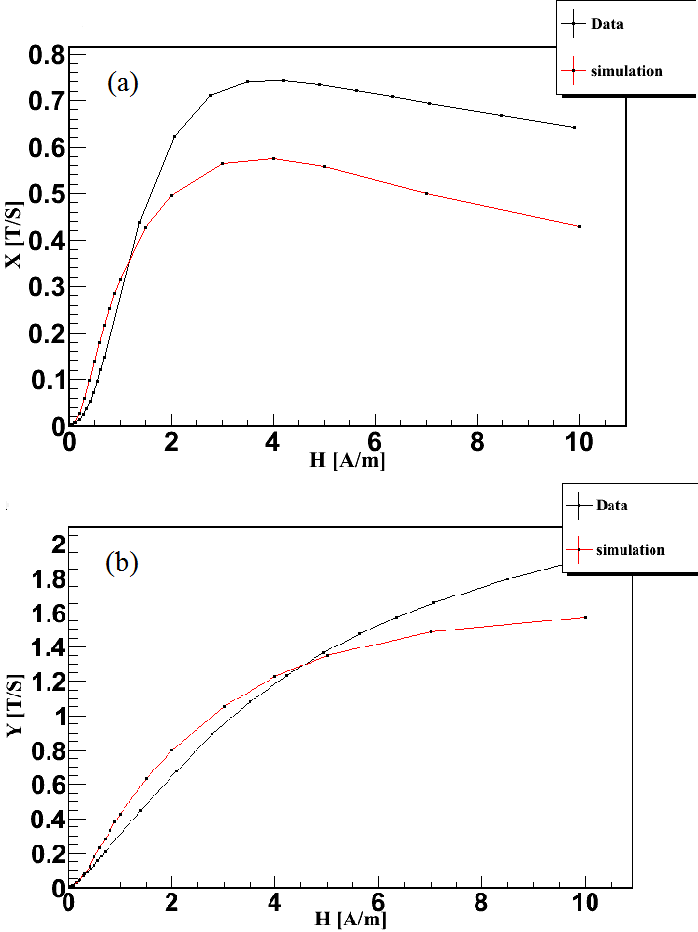
\includegraphics[width=0.5\textwidth]{data_and_simulation3.PNG}
    \caption{These graphs represent the sense voltage as a function of applied $H$ field at 1 Hz. Graph (a) shows the out-of-phase component $X$ of the measured sense voltage as well as the simulation. Graph (b) shows the in-phase component $Y$ of the signal and its simulation.}
    \label{fig:data_and_simulation}
    \end{center}
\end{figure} 

\subsubsection{Systematic Errors}

% Need list
% Please place here
%
% 1.  Focus on unique ones:
% - motion of wires (done)
% - degaussing, how done, and general observations (done)
% - resistance of wires (done)
% - different numbers of turns on primary/secondary  (Taraneh: talked about it earlier)
% - in-phase/out-of-phase components, how small should in-phase be? (Taraneh: talked about it)
% - background noise (done)
% - ...

% 2.  Or if there are any other ones that are from the same source
% (e.g. resistance of wire might be in this category) but the value is
% different for some reason

% 3.  Or if some are eliminated, it would be good to note here, for
% example, fluxgate systematics and some classes of motion systematics


The dominant source of systematic uncertainty in this method arises
from the properties of witness cylinders. 

%motion of wires
Since the coils were wound by hand the spacing between each loop of wire was not precise and it might lead to the motion of the wires during data acquisition. Although it might effect the measurement results, there was no way to address this systematic effect.


%degaussing
Some measurements conducted to study the effect of magnetization on the measured sense voltage. Degaussing
(idealizing) magnetic shields means to saturate the shields by
applying a very large magnetic field and then slowly turn the
applied field down to zero. In our case it was done by a C code controlling the lock-in amplifier. A sine wave with a known frequency, typically 1~Hz was applied on the primary coil. The minimum voltage change in a lock-in amplifier is 2~mV. The applied voltage was changing from 5~V to 4~mV which is the minimum possible voltage on a lock-in amplifier. It was also possible to adjust the speed of the degaussing as a time delay was implemented in the code.
The voltage was then increased to reach the typical $H$ field.
A comparison between the $X$ and $Y$ components of the sense voltage before and after degaussing was then made to study the effect.
In most cases, degaussing helped to
increase both the $X$ and $Y$ signal and hence $\mu$ although it did not change its temperature dependence significantly. Very long degaussing has a reverse effect on the measured signal.
% But it didn't change its temperature dependence significantly.  Poor
% degaussing could result in initial slopes that were large for a
% while?


%resistance of wire
To check the stability of the applied current on the primary coil, voltage across a 1~$\Omega$ temperature controlled resistor in series with the primary coil was measured. The result showed about 100~ppm/K changes in current.
%Taraneh: does this number make sense? I might need to double check it again.

%background noise
To reduce the background noise and
thermally isolate the witness cylinder, some measurements were done by
placing the witness cylinder inside the prototype passive shield. The
results did not show a significant change.


Saturation and magnetization of the witness cylinders and the nonlinearity of $/mu$ in general had
a considerable effect on the measured signal. Despite of the
consistent general trend of $B(T)$, different witness cylinders tend
to behave differently under similar conditions. 












%\begin{itemize}
%\item Describe experimental setup and important consdierations (e.g. relationship of data to effective $%\mu$)
%\item Explain B, H, f, and dominant systematic effects.
%\item Understanding in terms of Jiles-Atherton.  Complications that
 % this does not translate well into ``$\mu$''.
%\item One data graph?  (Perhaps the Jiles-Atherton one?)
%\item State overall result and systematic error.
%\end{itemize}
%%%%%%%%%%%%%%%%%%%%%%%%%%%%%%%%%%%%%%%%%%%%%%%%%%%%%%%%%%%%%%%%%%%%%%
% Taraneh, can you write text up to this point?
%%%%%%%%%%%%%%%%%%%%%%%%%%%%%%%%%%%%%%%%%%%%%%%%%%%%%%%%%%%%%%%%%%%%%%
